\section{Experiment}

% image in groupc
\begin{figure*}

    \centering
    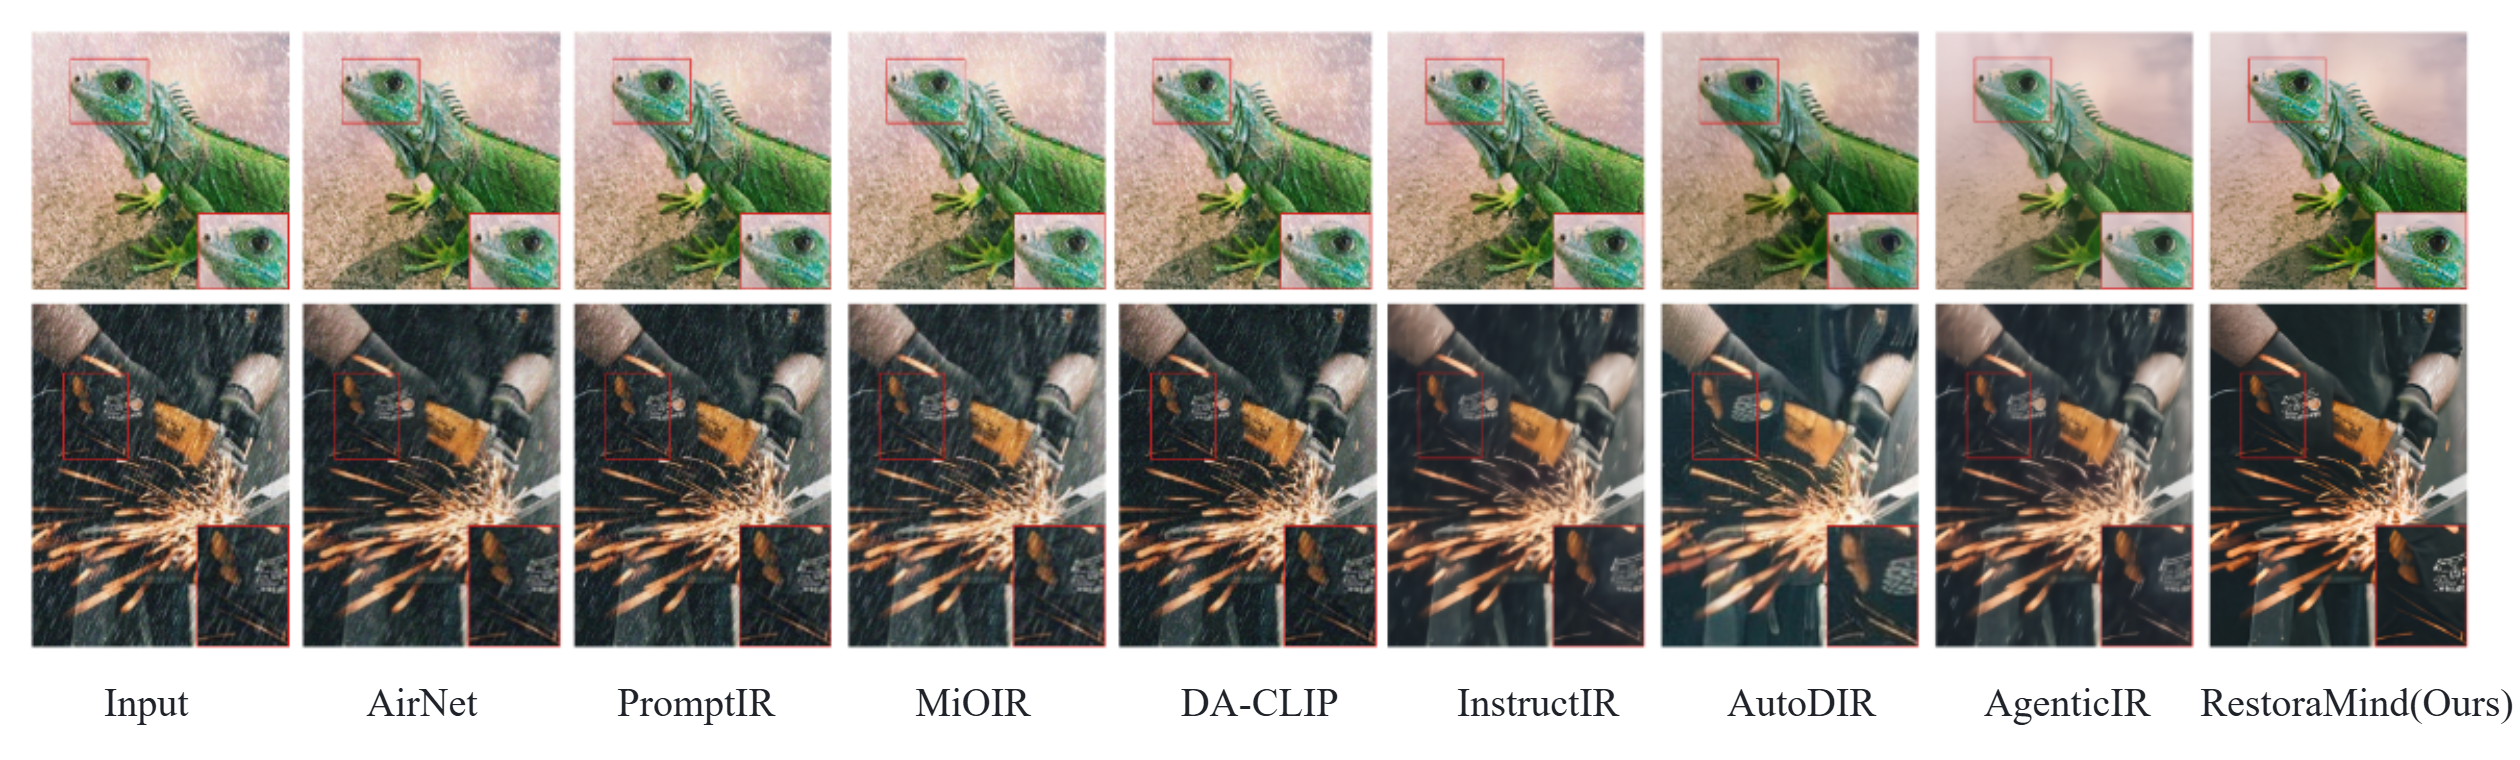
\includegraphics[width=\linewidth]{sec/fig/sub4/fig1.png}
    \caption{\textbf{Qualitative comparison } of various image restoration methods on Group C test images. RestoraMind (Ours) effectively recovers fine details like hair texture and sparks, outperforming baselines in addressing complex degradations.}
    \label{fig:3}
\end{figure*}


% 我们采用混合降质方法构建研究数据集。在实验部分，我们首先搭建测试数据集。我们设计了一个包含多种组合并且施加强度随机的测试集。该测试集所拥有的组合能够涵盖绝大部分场景，我们构建的组合数远超AgenticIR的16种。如3.x所描述，我们从unsplash-lite种获取7000张高质量图片，按照4：1比例划分训练集和验证集，并对每张图片施加2~3种降质
\subsection{Implementation Details}
\noindent\textbf{Dataset.}
To train the RestoraMind policy network, we constructed a new large-scale mixed-degradation dataset. We collected over 7,000 high-quality images from the Unsplash-lite dataset. To simulate complex blind restoration scenarios, we followed a sophisticated degradation pipeline, applying a random combination of 2 to 3 degradations with randomized intensities to each clean image. Our degradation library includes eight primary distortion types: haze, rain, defocus blur, low resolution, motion blur, low light, JPEG compression, and noise.
% To comprehensively evaluate the performance of our trained model, we adopt six key image quality metrics: three full-reference metrics, PSNR, SSIM (Wang et al., 2004), and LPIPS (Zhang et al., 2018), as well as three no-reference metrics, MANIQA (Yang et al., 2022), CLIP-IQA (Wang et al., 2023), and MUSIQ (Ke et al., 2021).

% \noindent\textbf{Training strategy.}
% RestoraMind involves fine-tuning the Q-Insight model, which itself is an RL-trained large multimodal model derived from Qwen2.5-VL-7B-Instruction~\cite{bai2025qwen2}. The model is fine-tuned for 10 epochs using the GRPO algorithm~\cite{Shao2024DeepSeekMathPT}. For optimization, the AdamW optimizer is used with $\beta_1=0.9$, $\beta_2=0.999$, a weight decay of 0.01, and a constant learning rate of 1e-6. 
% \textbf{ToolBox}
% The proposed RestoraMind agent addresses general image restoration by learning to select specialized tools from a predefined toolbox, which constitutes its discrete action space. This toolbox comprises pre-trained specialist models designed for low-level vision. It covers seven primary degradation categories, including Denoising, Deblurring (motion and defocus), Dehazing, Deraining, Super-Resolution, Low-Light Enhancement, and JPEG Artifact Removal. A complete and detailed inventory of all tools is provided in Appendix xx (see Table xx).

RestoraMind involves fine-tuning the Q-Insight model, which itself is an RL-trained large multimodal model derived from Qwen2.5-VL-7B-Instruction~\cite{bai2025qwen2}. The model is fine-tuned for 10 epochs using the GRPO algorithm~\cite{Shao2024DeepSeekMathPT}. For optimization, the AdamW optimizer is used with $\beta_1=0.9$, $\beta_2=0.999$, a weight decay of 0.01, and a constant learning rate of $1 \times 10^{-6}$. 
\textbf{ToolBox}
The proposed RestoraMind agent addresses general image restoration by leveraging the Q-Insight model to learn policies for selecting specialized tools from a predefined toolbox. This toolbox defines its discrete action space and comprises pre-trained specialist models tailored for low-level vision tasks. The tools correspond to seven primary degradation categories, including Denoising, Deblurring (motion and defocus), Dehazing, Deraining, Super-Resolution, Low-Light Enhancement, and JPEG Artifact Removal. A complete and detailed inventory of all tools is provided in Appendix xx (see Table xx).

%表1 总表 指标对比
\begin{table*}[h!]
\centering
\caption{\textbf{Quantitative comparison with state-of-the-art image restoration methods.} We compare RestoraMind to leading All-in-One models (AirNet, PromptIR) and Agentic methods (AgenticIR) across three degradation types. The results show that Agentic models (ours and AgenticIR) do much better than All-in-One models on perceptual metrics. RestoraMind also clearly outperforms AgenticIR on all No-Reference (NR) metrics, showing that it improves human-aligned perceptual quality, not just pixel-level accuracy.}
\label{tab:performance_comparison_v2}
\begin{tabular}{llcccccc}
\toprule
Degradations & Method & PSNR$\uparrow$ & SSIM$\uparrow$ & LPIPS$\downarrow$ & MANIQA$\uparrow$ & CLIP-IQA$\uparrow$ & MUSIQ$\uparrow$ \\
\midrule
\multirow{8}{*}{Group A}
& AirNet & 19.13 & 0.6019 & 0.4283 & 0.2581 & 0.3930 & 42.46 \\
& PromptIR & 20.06 & 0.6088 & 0.4127 & 0.2633 & 0.4013 & 42.62 \\
& MiOIR & 20.84 & 0.6558 & 0.3715 & 0.2451 & 0.3933 & 47.82 \\
& DA-CLIP & 19.58 & 0.6032 & 0.4266 & 0.2418 & 0.4139 & 42.51 \\
& InstructIR & 18.03 & 0.5751 & 0.4429 & 0.2660 & 0.3528 & 45.77 \\
& AutoDIR & 19.64 & 0.6286 & 0.3967 & 0.2500 & 0.3767 & 47.01 \\
& AgenticIR & \textbf{21.04} & \textbf{0.6818} & 0.3148 & 0.3071 & 0.4474 & 56.88 \\
& Restoramind & 19.57 & 0.6421 & \textbf{0.3086} & \textbf{0.3471} & \textbf{0.4824} & \textbf{60.80} \\
\midrule
\multirow{8}{*}{Group B}
& AirNet & 19.31 & 0.6567 & 0.3670 & 0.2882 & 0.4274 & 47.88 \\
& PromptIR & 20.47 & 0.6704 & 0.3370 & 0.2893 & 0.4289 & 48.10 \\
& MiOIR & \textbf{20.56} & 0.6905 & 0.3243 & 0.2638 & 0.4330 & 51.87 \\
& DA-CLIP & 18.56 & 0.5946 & 0.4405 & 0.2435 & 0.4154 & 43.70 \\
& InstructIR & 18.34 & 0.6235 & 0.4072 & 0.3022 & 0.3790 & 50.94 \\
& AutoDIR & 19.90 & 0.6643 & 0.3542 & 0.2534 & 0.3986 & 49.64 \\
& AgenticIR & 20.55 & \textbf{0.7009} & \textbf{0.3072} & 0.3204 & 0.4648 & 57.57 \\
& Restoramind & 19.98 & 0.6732 & 0.3161 & \textbf{0.3439} & \textbf{0.4762} & \textbf{59.19} \\
\midrule
\multirow{8}{*}{Group C}
& AirNet & 17.95 & 0.5145 & 0.5782 & 0.1854 & 0.3113 & 30.12 \\
& PromptIR & 18.51 & 0.5166 & 0.5756 & 0.1906 & 0.3104 & 29.71 \\
& MiOIR & 15.63 & 0.4896 & 0.5376 & 0.1717 & 0.2891 & 37.95 \\
& DA-CLIP & 18.53 & 0.5320 & 0.5335 & 0.1916 & 0.3476 & 33.87 \\
& InstructIR & 17.09 & 0.5135 & 0.5582 & 0.1732 & 0.2537 & 33.69 \\
& AutoDIR & 18.61 & 0.5443 & 0.5019 & 0.2045 & 0.2939 & 37.86 \\
& AgenticIR & \textbf{18.82} & 0.5474 & 0.4493 & 0.2698 & 0.3948 & 48.86 \\
& Restoramind & 18.44 & 0.5376 & \textbf{0.4233} & \textbf{0.2730} & \textbf{0.3996} & \textbf{50.32} \\
\bottomrule
\end{tabular}
\end{table*}
% table end
% image in real data
\begin{figure*}
    \centering
    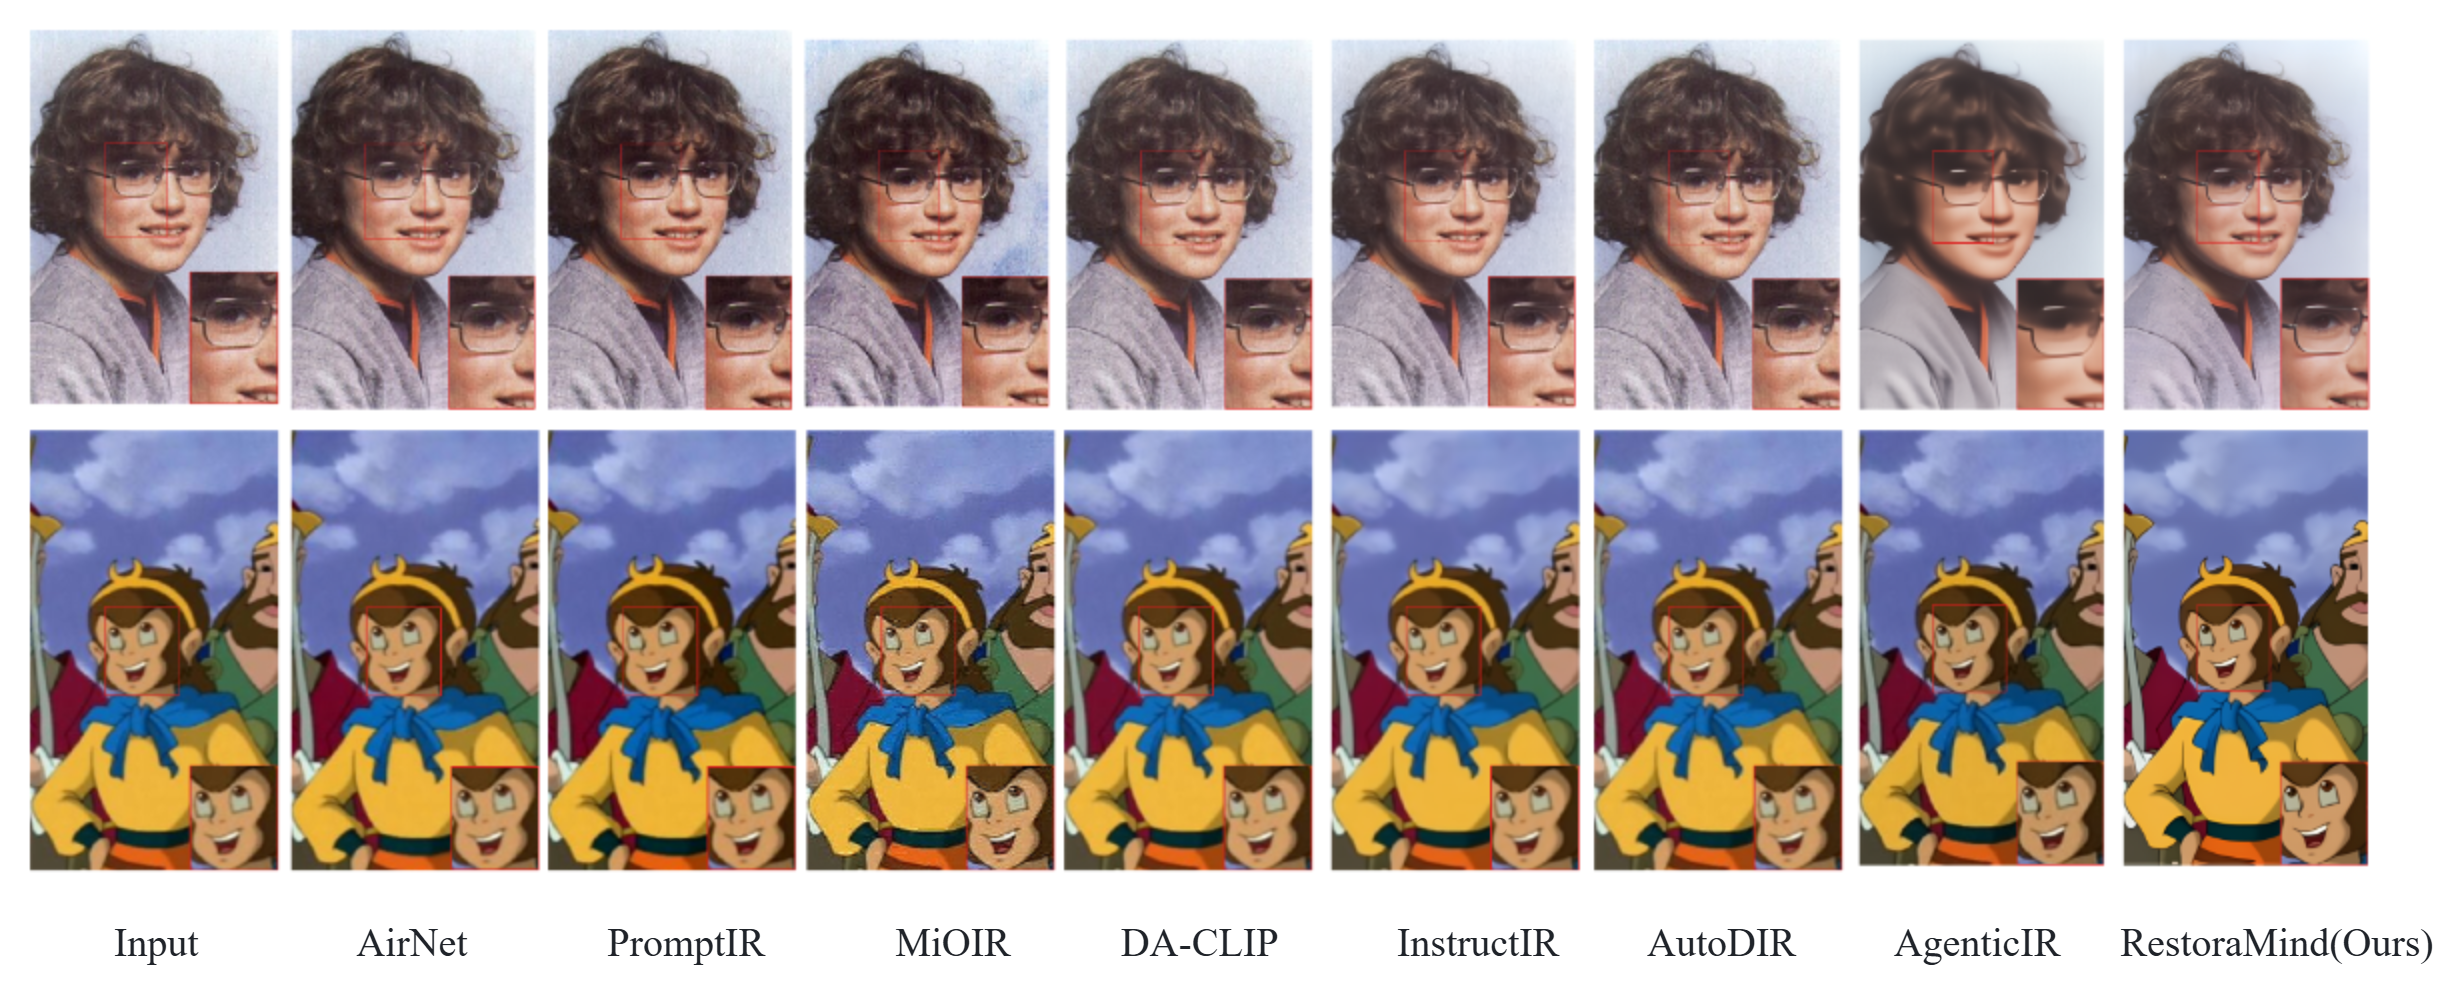
\includegraphics[width=\linewidth]{sec/fig/sub4/fig2.png}
    \caption{\textbf{Qualitative comparison on real-world scenarios.} Visual results on old photographs (top) and cartoon images (bottom) demonstrate the robustness of RestoraMind. While baselines often struggle with domain gaps—leaving distinct noise patterns.RestoraMind demonstrates superior generalization.Our method adaptively restores semantic clarity and natural textures, effectively handling unknown degradations across diverse domains.}
    \label{fig:4}
\end{figure*}

\noindent\subsection{Image quality comparison.}
% We report the quantitative comparison of RestoraMind against SOTA methods across three degradation groups in \cref{tab:performance_comparison_v2}. A primary observation is the clear superiority of the Agentic paradigm over All-in-One approaches. ~\cite{li2022all,potlapalli2023promptir,kong2024towards,luo2023controlling,conde2024instructir,jiang2024autodir,zhu2024intelligent} As shown in the table, both RestoraMind and AgenticIR significantly outperform All-in-One baselines such as AirNet, PromptIR, and MiOIR on most metrics, especially on critical perceptual ones like LPIPS, MANIQA, and MUSIQ. The results clearly reveal a fundamental advantage in RestoraMind's optimization objective: it successfully avoids overfitting to conventional fidelity metrics, achieving superior optimization for human-centric visual perception instead.
We report the quantitative comparison of RestoraMind against SOTA methods across three degradation groups in \cref{tab:performance_comparison_v2}. A primary observation is the clear superiority of the Agentic paradigm over All-in-One approaches. ~\cite{li2022all,potlapalli2023promptir,kong2024towards,luo2023controlling,conde2024instructir,jiang2024autodir,zhu2024intelligent} As shown in the table, both RestoraMind and AgenticIR significantly outperform All-in-One baselines such as AirNet, PromptIR, and MiOIR on most metrics. This holds especially for critical perceptual ones, such as LPIPS, MANIQA, and MUSIQ. The results clearly reveal a fundamental advantage in RestoraMind's optimization objective. It successfully avoids overfitting to conventional fidelity metrics and achieves superior optimization for human-centric visual perception.

% RestoraMind demonstrates a decisive and consistent superiority across the full suite of No-Reference (NR) perceptual metrics. Despite trailing slightly on LPIPS in Group B, our model consistently outperforms AgenticIR on MANIQA~\cite{yang2022maniqa}, CLIP-IQA~\cite{wang2023exploring}, and MUSIQ\cite{ke2021musiq} across all three degradation groups. This is a critical finding: NR metrics are designed to model human judgment without access to a ground truth, making them a far more authentic and challenging proxy for real-world quality. RestoraMind's consistent victory here proves that our end-to-end RL agent successfully learned to optimize for this higher-level, more human-aligned objective, rather than mechanically fitting to pixel-level ground truths.

RestoraMind demonstrates decisive, consistent superiority across all No-Reference (NR) perceptual metrics. While it trails slightly on LPIPS in Group B, our model consistently outperforms AgenticIR on MANIQA~\cite{yang2022maniqa}, CLIP-IQA~\cite{wang2023exploring}, and MUSIQ\cite{ke2021musiq} in all three degradation groups. This is critical: NR metrics model human judgment without ground truth, serving as a more authentic and challenging proxy for real-world quality. RestoraMind's consistent victory demonstrates that our end-to-end RL agent has learned to optimize for this higher-level, human-aligned objective, rather than simply fitting to pixel-level ground truths.



% image result
Qualitative comparisons in \cref{fig:3} and \cref{fig:4} visually corroborate these findings. As shown in \cref{fig:3}, All-in-One baselines (e.g., AirNet, PromptIR) often struggle to disentangle complex degradations, resulting in residual artifacts (e.g., rain streaks) or excessive over-smoothing. In contrast, RestoraMind recovers fine high-frequency details, such as skin texture and sparks, without the over-sharpening artifacts occasionally observed in AgenticIR.
Furthermore, \cref{fig:4} validates the robustness of RestoraMind on real-world scenarios, including old photos and cartoons. While baselines like DA-CLIP often fail to generalize due to domain gaps, leaving distinct noise patterns, our end-to-end RL policy enables RestoraMind to adaptively restore semantic clarity and natural textures even under unknown degradations.


Crucially, RestoraMind achieves this superior quality while realizing a significant efficiency gain. AgenticIR relies on an expensive, trial-and-error search to reach its "High-PSNR" result, whereas our end-to-end RL agent significantly shortens this process (Table.~\ref{tab:performance_comparison_v2}). In conclusion, RestoraMind validates the superiority of an end-to-end RL framework for Agentic IR. It not only significantly alleviates the critical efficiency bottleneck of search-based methods but, more importantly, strikes an excellent trade-off between restoration quality (especially perceptual quality) and inference efficiency, rendering it a far more practical and human-aligned solution.

\begin{figure*}[htbp]
    \centering
    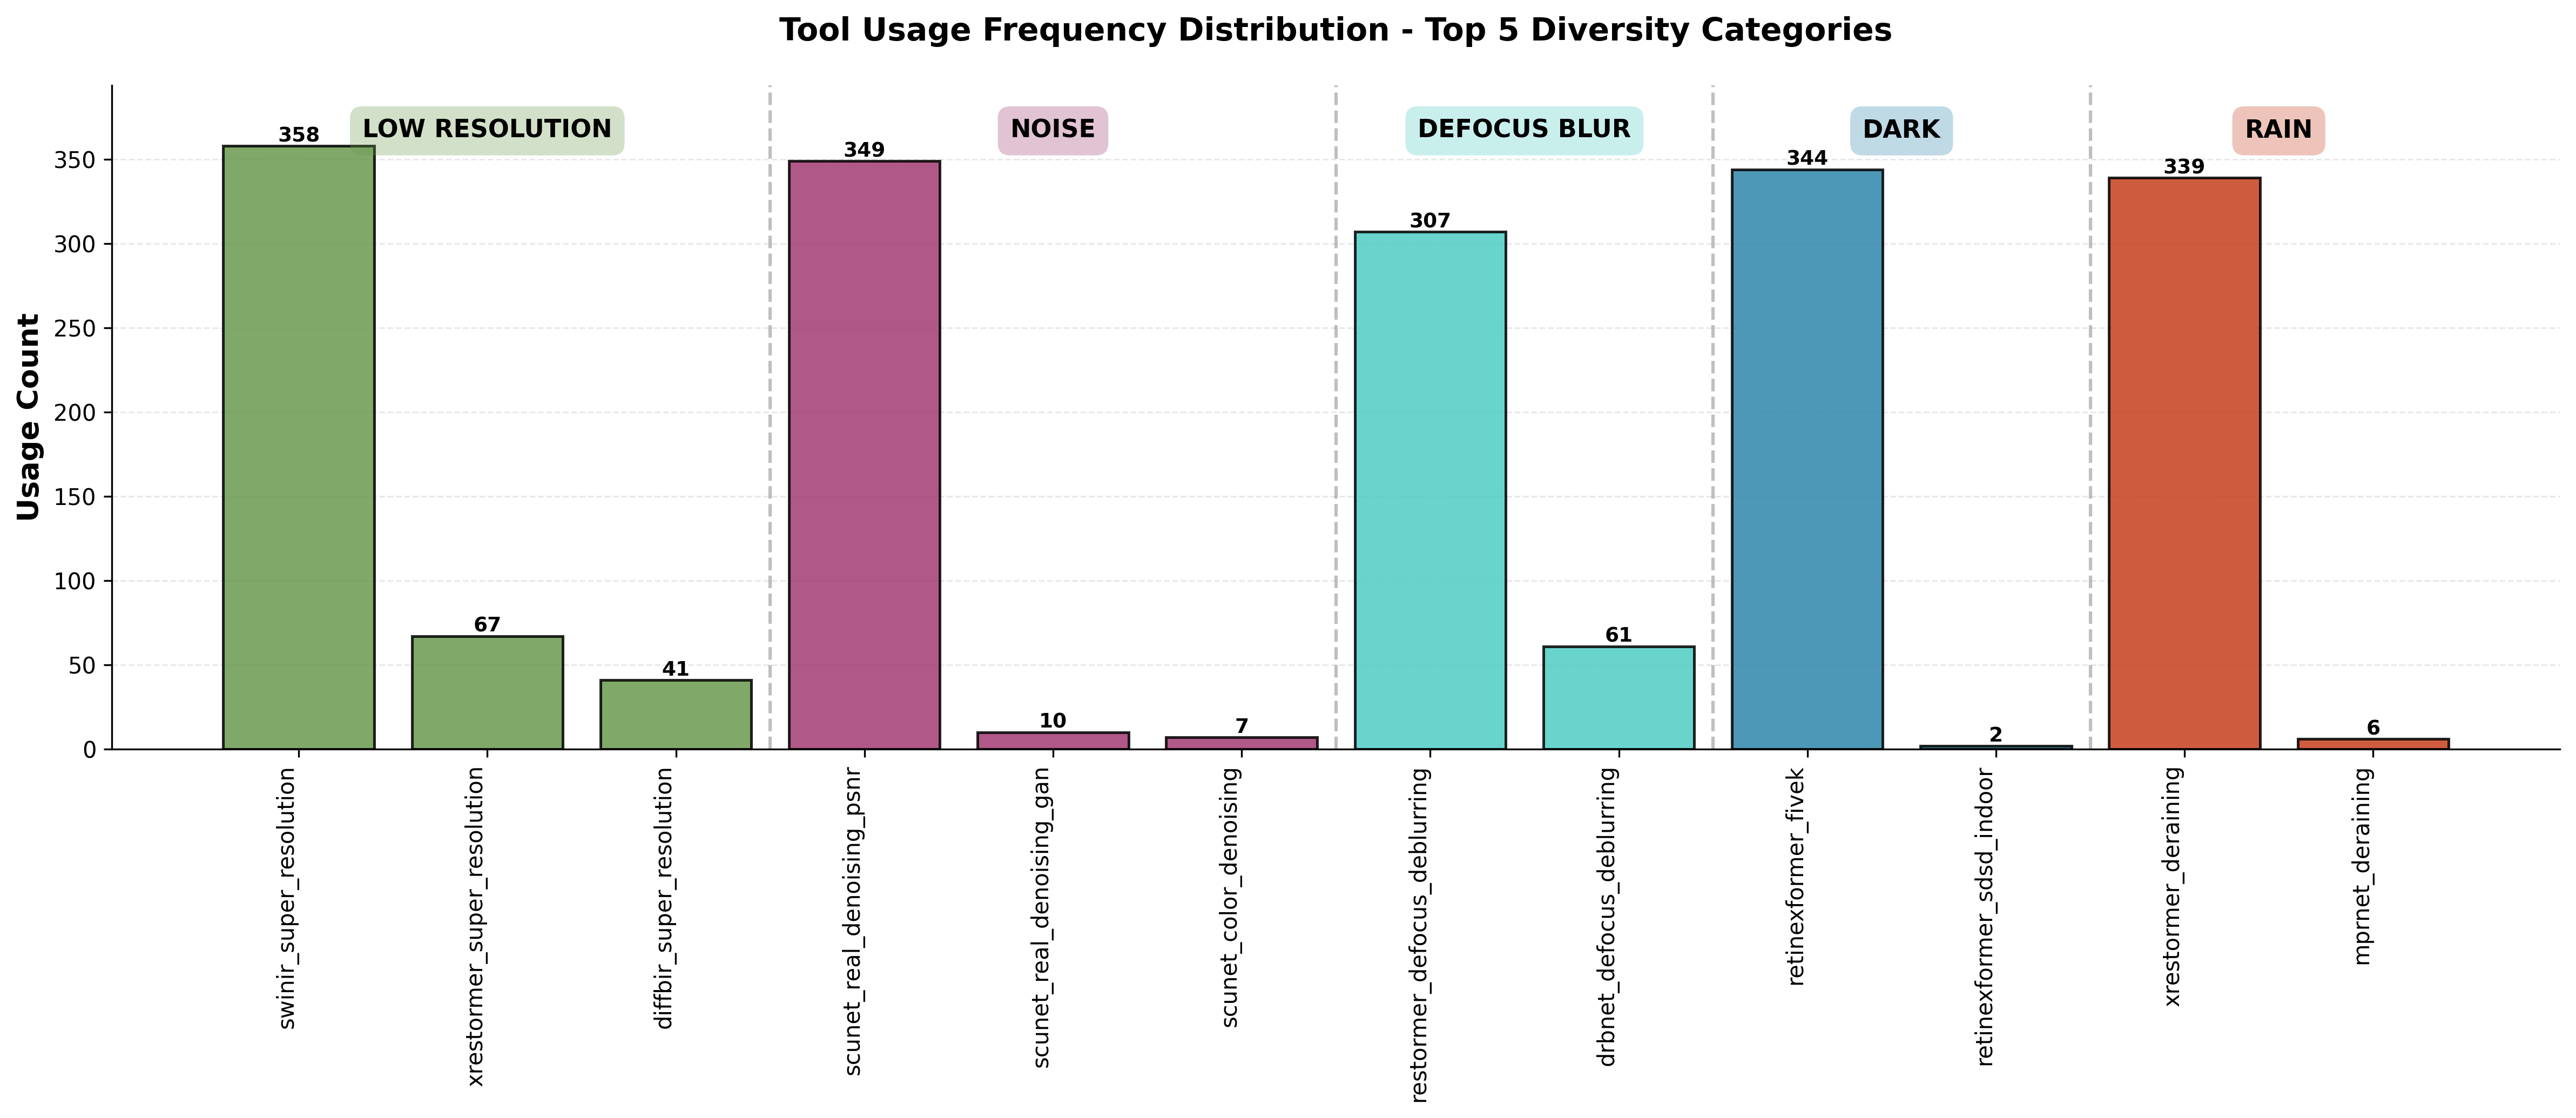
\includegraphics[width=1.0\linewidth]{sec/fig/tool_usage_histogram_top5_diversity.png}
    \caption{\textbf{Tool Usage Frequency Distribution.} The chart illustrates the agent's tool invocation frequency across the top five degradation categories. This distribution demonstrates that while the agent identifies dominant, general-purpose tools (e.g., swinir super resolution and  scunet real denoising psnr), it does not collapse into a trivial policy. The significant, non-zero usage of alternative tools (e.g., xrestormer super resolution and  drbnet defocus deblurring) validates that RestoraMind leverages image statistics  for fine-grained, adaptive tool selection.}
    \label{fig:histogram}
\end{figure*}

\noindent\subsection{Restoration Efficiency Comparison}
As shown in Table~\ref{tab:2speed}, our end-to-end RestoraMind agent demonstrates a decisive advantage in efficiency. The search-based AgenticIR incurs a high computational cost to find its optimal solution, as it calls all tools capable of solving each degradation type, requiring xx seconds for average inference. In contrast, RestoraMind leverages its end-to-end trained policy, reducing the average inference time to xx seconds, a significant efficiency gain.
% 

\begin{table}[h!] % [h!] 
\centering
\caption{method compare}
\label{tab:time comparison}
\begin{tabular}{lcc}
\toprule
\textbf{Method} & \textbf{Time (s) $\downarrow$} & \textbf{Invocations $\downarrow$} \\
\midrule
AgenticIR     & 65.04                & 5.15                \\
\textbf{RestoraMind (Ours)} & \textbf{\textcolor{red}{xx}} & \textbf{\textcolor{red}{xx}} \\
\bottomrule
\end{tabular}
\label{tab:2speed}
\end{table}

\noindent\subsection{Analysis of Adaptive Tool Selection}
As illustrated in \cref{fig:histogram}, we observe that for each primary degradation category, the agent identifies a "dominant" tool. For instance, "swinir super Resolution" is invoked 358 times for Low Resolution, and "scunet real denoising psnr" is used 349 times for Noise. This indicates that RestoraMind correctly learns the general-purpose robustness and superior performance of these specific tools for the majority of cases.

However, the critical finding is that the agent does not converge to a trivial, fixed policy of exclusively using these dominant tools. The distribution shows a significant and non-trivial invocation count for alternative models. For example,  ”xrestormer super resolution“ is still selected 67 times for Low Resolution, and ”drbnet defocus deblurring“ is chosen 61 times over its dominant Restormer counterpart.

This diversified selection behavior strongly validates our hypothesis. It demonstrates that RestoraMind successfully leverages the incorporated image statistics as informative priors. Rather than adhering to a rigid rule, the agent makes content-aware decisions, adaptively switching to an alternative tool when its internal policy predicts a more favorable outcome based on the specific low-level characteristics of the input image. This confirms the agent's ability to master the complementary strengths of different tools within the same category, achieving a more intelligent and effective restoration process.


%表2 多工具直方图

%表3 速度对比

%表4 Qinsight调用工具 qwen调用工具 

%图3 sota图



%图4 real图




